%%--------------------------------Packages and stuff--------------------------------%%
\documentclass[11pt]{article}
\usepackage[utf8]{inputenc} %input type
\usepackage{siunitx}
\usepackage{lipsum} %for nonsense text
\usepackage{verbatim} %for multiline comments
\usepackage{fancyhdr} %header&footer
\usepackage{natbib} %bibliography
\usepackage{hyperref} %hyperlinks
\hypersetup{
     colorlinks   = true,
     citecolor    = black,
     urlcolor = black,
     linkcolor = black
}
\usepackage[nottoc,notlot,notlof]{tocbibind} %for showing  bibliography in toc
\usepackage{listings}
\usepackage{textcomp}
\usepackage{mathtools}
\usepackage{enumitem}
\setitemize{noitemsep,topsep=0pt,parsep=0pt,partopsep=0pt}
\renewcommand\labelitemi{\scriptsize$\bullet$}
\usepackage{array}
\newcolumntype{N}{@{}m{0pt}@{}}
\usepackage{indentfirst} %indent first paragraph
\setlength{\parindent}{4mm}

\usepackage{datetime}
\newdateformat{monthyeardate}{%
\THEYEAR}

\renewcommand{\figurename}{Slika}
\renewcommand\bibname{Literatura}

%%--------------------------------Figures setup--------------------------------%%
\usepackage{graphicx} %for  images
\usepackage{grffile} %for pngs
\graphicspath{ {images/} } %images path
%%--------------------------------End of figures setup--------------------------------%%

%%--------------------------------Geometry aka page layout setup--------------------------------%%
\usepackage{geometry} %geometry aka page layout
\geometry{
  a4paper,
  left=25mm,
  right=25mm,
  top=25mm,
  bottom=25mm,
  head=25mm
}

\setlength{\parindent}{1em}
%\setlength{\parskip}{1em}
%%--------------------------------End of geometry aka page layout setup--------------------------------%%

\usepackage{fontspec}
\usepackage{minted}

%%--------------------------------Caption setup--------------------------------%%
\usepackage{caption}
\DeclareCaptionStyle{mystyle}
  {format=plain,
    textformat=period,
    justification=RaggedRight,
    singlelinecheck=true,
  }% all captions are left aligned

\DeclareCaptionStyle{singlelinecentered}
  [justification=Centering]% centered if single line and no `singlelinecheck=false`
  {style=mystyle}% other captions are left aligned

\captionsetup{style=singlelinecentered}
%%--------------------------------End of caption setup--------------------------------%%

%%--------------------------------Title formatting--------------------------------%%
\usepackage{titlesec}
%%-----Spacing-----%%
\titleformat{\section}[hang]{}{\thesection}{0.4em}{}
\titleformat{\subsection}[hang]{}{\thesubsection}{0.4em}{}
\titleformat{\subsubsection}[hang]{}{\thesubsubsection}{0.4em}{}
\titleformat{\paragraph}[hang]{}{\theparagraph}{0.4em}{}
\titlespacing{\section}{0mm}{5mm}{2mm}
\titlespacing{\subsection}{0mm}{5mm}{2mm}
\titlespacing{\subsubsection}{0mm}{5mm}{2mm}
\titlespacing{\paragraph}{0mm}{5mm}{2mm}

%%-----Font-----%%
\titleformat*{\section}{\Large\bfseries\sffamily}
\titleformat*{\subsection}{\large\bfseries\sffamily}
\titleformat*{\subsubsection}{\normalsize\bfseries\sffamily}
\titleformat*{\paragraph}{\normalsize\bfseries\sffamily}
%%--------------------------------End of Title formatting--------------------------------%%

%%--------------------------------ToC setup--------------------------------%%
\usepackage{tocloft}
\setcounter{secnumdepth}{5}
\setcounter{tocdepth}{5}
\renewcommand\cftsecleader{\cftdotfill{\cftdotsep}}
\setlength{\cftfigindent}{0pt}
\setlength{\cfttabindent}{0pt}
%\newcommand{\cfttocnumwidth}{}
\renewcommand{\listfigurename}{\sffamily{\Large{Kazalo slik}}}
\renewcommand{\listtablename}{\sffamily{\Large{Kazalo tabel}}}
\renewcommand{\contentsname}{Kazalo}
\renewcommand{\cfttoctitlefont}{\Large\bfseries\sffamily}
%\setlength{\cfttocnumwidth}{1mm}
%%--------------------------------End of ToC setup--------------------------------%%

%%--------------------------------Acronyms and glossaries setup--------------------------------%%


%\usepackage[acronym, toc]{glossaries}
\usepackage[acronym]{glossaries}
\makeglossaries
%%--------------------------------Acronyms--------------------------------%%
\newacronym{ssh}{SSH}{Secure Shell}
\newacronym{lcd}{LCD}{Liquid Crystal Display}
\newacronym{gpio}{GPIO}{General-purpose input/output}
%%--------------------------------End of Acronyms--------------------------------%%

%%--------------------------------Glossary--------------------------------%%

%%--------------------------------End of Glossary--------------------------------%%
%%--------------------------------End of acronyms and glossaries setup--------------------------------%%

%%--------------------------------Custom commands--------------------------------%%
\newcommand{\shellcmd}[1]{\\\indent\indent\texttt{\normalsize\$ #1}\\}
\newcommand{\shellcmdn}[1]{\\\texttt{\normalsize\$ #1}\\}
\newcommand{\source}[2]{\caption{#1}\vspace{-1.5mm}{\tiny{Vir: \url{{#2}}}} }
\newcommand{\numpara}[1]{\paragraph{{#1}}\mbox{}\vspace{0mm}}
%%--------------------------------End of Custom commands--------------------------------%%

%%--------------------------------End of packages and stuff--------------------------------%%

%%--------------------------------Beginning of the document--------------------------------%%
\begin{document}

\renewcommand{\theFancyVerbLine}{
  \sffamily\textcolor[rgb]{0.5,0.5,0.5}{\scriptsize\arabic{FancyVerbLine}}}

\begin{titlepage}
\thispagestyle{empty}
   \center
   \fancyhead{}
   \large{Šolski center Celje, Srednja šola za kemijo, elektrotehniko in računalništvo}\\[1.5cm]
   \vspace*{\fill}
   \begin{center}
   \Huge{\bfseries Pametna garažna vrata}\\
   \vspace{1mm}
   \large{raziskovalna naloga}
   \end{center}
   \vspace*{\fill}
   	%------------------------------------------------
	%	Author(s)
	%------------------------------------------------

	\begin{minipage}{0.4\textwidth}
		\begin{flushleft}
		\vspace{4.5mm}
			\large
			\texttt{Avtor}\\
			Boštjan \textsc{Planko}, R-4.A \\ %Author's name
			%\vspace{0.2cm}
			%\texttt{Submission date} \\
			%\large{December 7, 2017}
		\end{flushleft}
	\end{minipage}
	~
	%------------------------------------------------
	%	Supervisor(s)
	%------------------------------------------------
	\begin{minipage}{0.5\textwidth}
		\begin{flushright}
			\large
			\texttt{Mentor}\\
			Borut \textsc{Slemenšek},  univ. dipl. inž % Supervisor's name
		\end{flushright}
	\end{minipage}
	~
	%------------------------------------------------
	%	Date
	%------------------------------------------------
	\begin{minipage}{0.5\textwidth}
		\begin{center}
		    \vspace{5mm}
		    Mestna občina Celje, Mladi za Celje\\
			\large{Celje, marec \monthyeardate\today}
		\end{center}
	\end{minipage}
	\fancyfoot{}
\end{titlepage}
%%--------------------------------End of title page--------------------------------%%

%%--------------------------------Beginning of abstract--------------------------------%%
\newpage
\thispagestyle{empty}
\section*{Povzetek}
Raziskoval sem podrčje elektronike in avtomizacije. Glavno vprašanje razsikovalne naloge je bilo ali je mogoče avtomatizirati garažna vrata z Raspberry Pi računalnikom. Potrebno znanje, ki ga še nisem imel, sem pridobil z metodo analize dokumentov in metodo eksperimenta. Tekom nastajanja projekta sem prišel do zaključka, da je osnovna ideja sicer enostavna, v praksi pa stvari zelo hitro postanejo zelo kompleksne. Rezultat moje raziskovalne naloge je delujoč prototip, na katerem delujejo vse osnovne funkcije. Je dober temelj za nadaljnji razvoj in širitev projekta.
\section*{Summary}
I was researching the field of electronics and automation. The main goal of this paper was finding out if it is possible to automate garage doors using Raspberry Pi. I had to analyze a lot of documentation to get the knowledge that was required to finish my project. I also had to experiment quite a lot. In the end, I came to the conclusion that the basic idea for my project is quite simple. Despite that, things can get really complicated really fast. The end result of my work is a working prototype that has a lot of possibilities to expand the project even further.
\section*{Ključne besede}
raspberry pi, senzorji, python, raspbian, avtomizacija

\printglossary[type=\acronymtype,title={Kratice}]
%%--------------------------------End of abstract--------------------------------%%

%%--------------------------------Beginning of ToC--------------------------------%%
\renewcommand{\baselinestretch}{0.90}\normalsize
\newpage
\pagenumbering{gobble}
\thispagestyle{empty}
\tableofcontents
\newpage
\listoffigures
\renewcommand{\baselinestretch}{1.0}\normalsize
%%--------------------------------End of ToC--------------------------------%%
\newpage

%%--------------------------------Beginning of head & foot--------------------------------%%
\pagestyle{fancy}
\fancyhead{}
\fancyhead[C]{Pametna garažna vrata}
\fancyfoot{}
\fancyfoot[C]{\thepage}
%%--------------------------------End of head & foot--------------------------------%%

%%--------------------------------Beginning of Section 1 aka Intro--------------------------------%%

\newpage
\pagenumbering{arabic}
\setcounter{page}{6}
\section{Uvod}
\subsection{Opis problema}
Problem današnjih garažnih vrat je, da jih je običajno možno odpreti samo na dva načina: s priloženim daljincem ali s tipko, običajno nameščeno na notranji strani garažnih vrat. Če želimo garažna vrata odpreti moramo torej biti v garaži ali pa moramo imeti pri sebi daljinec. To pa je v vsakdanjem življenju nepraktično, sploh v primeru, ko pri hiši živi veliko ljudi, vsi pa rabijo dostop do garaže.

V tej nalogi bom predstavil svojo idejo, pametna garažna vrata, kot sem si jih zamislil in poskušal realizirati.

\subsection{Hipoteze}
Za raziskovalno nalogo sem si postavil naslednje hipoteze:
\begin{enumerate}
  %\setlength\itemsep{0.5mm}
    \item Garažna vrata bo možno upravljati s telefonom.
    \item Garažna vrata bo možno upravljati preko spletne strani.
    \item Raspberry Pi bo spremljal, ali je avto v garaži ali ne, in glede na to samodejno zapiral garažna vrata.
    \item Raspberry Pi bo spremljal temperaturo v garaži in jih samodejno zaprl v primeru prenizke ali previsoke temperature.
    \item Raspberry Pi nas bo s potisnimi obvestili obveščal o spremembi stanja garažnih vrat.
    \item Raspberry Pi bo beležil, kdo in kdaj je aktiviral garažna vrata.
    \item Uporabnik bo imel možnost preklicati samodejno zapiranje vrat.
\end{enumerate}

\section{Raziskovalne metode}
Med raziskovanjem sem uporabil kombinacijo različnih metod, saj sem tako najlaže prišel do rešitve problema.

Na začetku raziskovanja sem uporabljal predvsem metodo analize dokumentov. Prebral in preučil sem veliko dokumentacije in objav na forumih. Tako sem pridobil osnovno podlago za začetek dela na svojem projektu.

Pri programiranju in sestavljanju prototipa sem uporabil predvsem metodo eksperimenta. Preizkusil sem veliko različnih konfiguracij in programskih rešitev, na koncu pa sem izbral tiste, ki so se mi zdele najbolj optimalne.
\newpage

\section{Izbira komponent}
  Ker ne potrebujem veliko precesorske moči, hkrati pa želim, da je moj projekt kar se da kompakten sem za krmilnik izberal Raspberry Pi Zero W. To je najmanjša verzija Raspberry Pi-ja z že vgrajenim WiFi-jem in Bluetoothom. Slednja bosta pri projektu najverjetneje potrebna.

  Za upravljanje garažnih vrat bom uporabil 1-kanalni rele. Tega bom sprogramiral tako, da se bo obnašal kot tipka, tj. zaprl se bo za kratek časovni interval, prib. 0.5 s, nato pa se znova odprl. Nameščen bo v bližini že obstoječe tipke, ki se uporablja za upravljanje garažnih vrat. S to bo vezan vzporedno.

  Za spremljanje stanja garažnih vrat bom uporabil reed stikala, in sicer dve stikali in magnet. Stikali bosta nameščeni na ogrodje vrat, medtem ko bo magnet nameščen neposredno na garažna vrata.

  Za spremljanje temperature v garaži bom uporabil 1-Wire digitalni element DS18B20. Ta bo nameščen nekje v garaži, po možnosti meter od tal, na najmanj prepišnem mestu.

  Ultrazvočni senzor, s katerim bom preverjal je avto v garaži ali ne, bo nameščen ali na stropu garaže, najverjetneje kar na motorju garažnih vrat.

  Ker želim, da bo mogoče v garaži preveriti trenutno temperaturo in čas, bom uporabil tudi 16x2 \gls{lcd} zaslon.

  Poleg že naštetih komponent bo uporabil še dve LED diodi in dve tipki. Te bodo uporabljene paroma kot indikator stanja avta oziroma temperature v garaži. Če bo na primer garaža odprta in bo vanjo pripeljal avto, se bo pognal program, ki bo po določenem času samodejno zaprl vrata. Istočasno bo začela utripati ustrezna LED dioda, uporabnik pa bo imel s pritiskom tipke možnost, da prekliče samodejno zapiranje garaže. Pri temperaturi je namen LED diode in tipke enak, le da z njima spremljamo temperaturo v garaži.
\section{Priprava Raspberry Pi-ja}
 Da bom lahko uporabljal Raspberry Pi, moram najprej naložiti usterzen opreacijski sistem. Ker za svoj projekt ne potrebujem grafičnega vmesnika, na Raspberry Pi namestim Raspbian Lite. To storim tako, da iz uradne strani Raspberry Pi \cite{RPi_raspbian} prenesem Raspbian Stretch Lite. Nato sledim navodilom za namestitev \cite{RPi_install} operacijskega sistema na microSd kartico, ki jo nato vstavim v Raspberry Pi.

Ker do Raspberry Pi-ja že od samega začetka nimam dostopa preko tipkovnice, moram pred zagonom omogočiti še \gls{ssh} ter vnesti podatke, ki jih Raspberry Pi potrebuje za povezavo na WiFi dostopno točko. Da omogočim \gls{ssh}, na boot particijo microSD katrice dodam datoteko ssh. Da pa se bo Raspberry Pi lahko povezal na WiFi dostopno točko, moram na boot particiji ustvariti datoteko wpa\_supplicant.conf, v katero vnesem naslednje:
\newpage
\begin{minted}[mathescape,
               linenos,
               numbersep=5pt,
               gobble=0,
               frame=lines,
               framesep=2mm]{bash}

country=SI
ctrl_interface=DIR=/var/run/wpa_supplicant GROUP=netdev
update_config=1
network={
	ssid="imeDostopneTpočke"
	psk="geslo"
	key_mgmt=WPA-PSK
}
\end{minted}

Nato microSD kartico vstavim v Raspberry Pi in priključim napajanje.
\\

Nato se iz terminala na svojem računalniku preko \gls{ssh} povežem na Raspberry Pi:

\begin{minted}[mathescape,
               linenos,
               numbersep=5pt,
               gobble=0,
               frame=lines,
               framesep=2mm]{python}

ssh pi@IP_RaspberryPi #uporabnik pi, privzeto geslo pa je raspberry
\end{minted}

Ko je povezava vzpostavljena, uporabim ukaz \textit{passwd pi}, da spremenim geslo uporabnika pi.

Nato zaženem ukaz \textit{sudo raspi-config}
\begin{figure}[h]
\centering
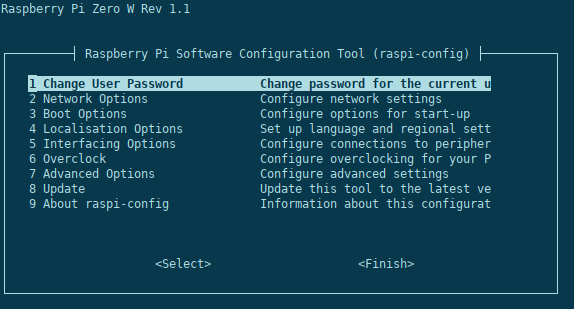
\includegraphics[width=10cm, height=5cm]{images/raspi-config.png}
\caption{Raspi-config: Glavni meni}
\end{figure}

Pojavi se meni, po katerem se premikam s pomočjo tipkovnice.

Tukaj nastavim vse potrebno:
\begin{itemize}
    \item hostname spremenim iz "raspberrypi" v "projectPi",
    \item časovno območje nastavim na Europe/Ljubljana,
    \item omogočim SPI, I2C in 1-Wire (vse to bom potreboval za priklop senzorjev),
    \item razširim datotečni sistem.
\end{itemize}

Preden namestim nove pakete, je potrebno sistem posodobiti:

\begin{minted}[mathescape,
               linenos,
               numbersep=5pt,
               gobble=0,
               frame=lines,
               framesep=2mm]{python}

sudo apt update && sudo apt upgrade -y
\end{minted}

Ker bom program za upravljanje garažnih vrat napisal v Pythonu, le tega namestim na Raspberry Pi:
\begin{minted}[mathescape,
               linenos,
               numbersep=5pt,
               gobble=0,
               frame=lines,
               framesep=2mm]{python}

sudo apt install python python-pip
\end{minted}

Ker bom uporabil tudi \gls{lcd}, moram namestiti še RPILCD knjižnico:

\begin{minted}[mathescape,
               linenos,
               numbersep=5pt,
               gobble=0,
               frame=lines,
               framesep=2mm]{python}

sudo pip install RPLCD
\end{minted}

S tem je priprava Raspberry Pi-ja zaključena.

\section{Priključitev komponent}
\subsection{Rele}
Priklop releja je zelo enostaven. Modul z relejem ima tri priključke: VCC, GND in IN1. VCC priključek povežem na 5 V pin. GND priključim na GND pin. Za IN1 izberem BMC pin 16.

\subsection{Reed stikali}
Priključitev reed stikal je v osnovi zelo enostavna. Paziti je treba, da imamo NO (Normally Open) in ne NC (Normally Closed) stikala. Nato en del stikala povežemo na 3.3 V, drugi del pa na enega izmed \gls{gpio} pinov. Prvo stikalo (garaža odprta) sem priklopil na BCM pin 5, drugega (garaža zaparta) pa na BCM pin 6.

Po priklopu, je treba paziti, da v programu ne pozabimo nastaviti pull-down uporov, oba pina pa morata biti nastavljena kot vhodna. Tako ima pin vrednost 1, če je stikalo zaprto in vrednost 0, če je stikalo odprto.

\subsection{Ultrazvočni senzor razdalje HC-SR04}
Ker sem ultrazvočni senzor razdalje na Raspberry Pi uporabljal prvič, sem si pomagal z vodičem na ModMyPi \cite{ModMyPi_us}.

Senzor ima štiri pine: VCC, GND, Trig, Echo. VCC povežem na 5 V. GND povežem na GND pin, Trig na BCM pin 11, Echo pa najprej preko \SI{1}{\kohm} upora na BCM pin 20, nato pa še preko \SI{2}{\kohm} na GND.
\begin{figure}[h]
\centering
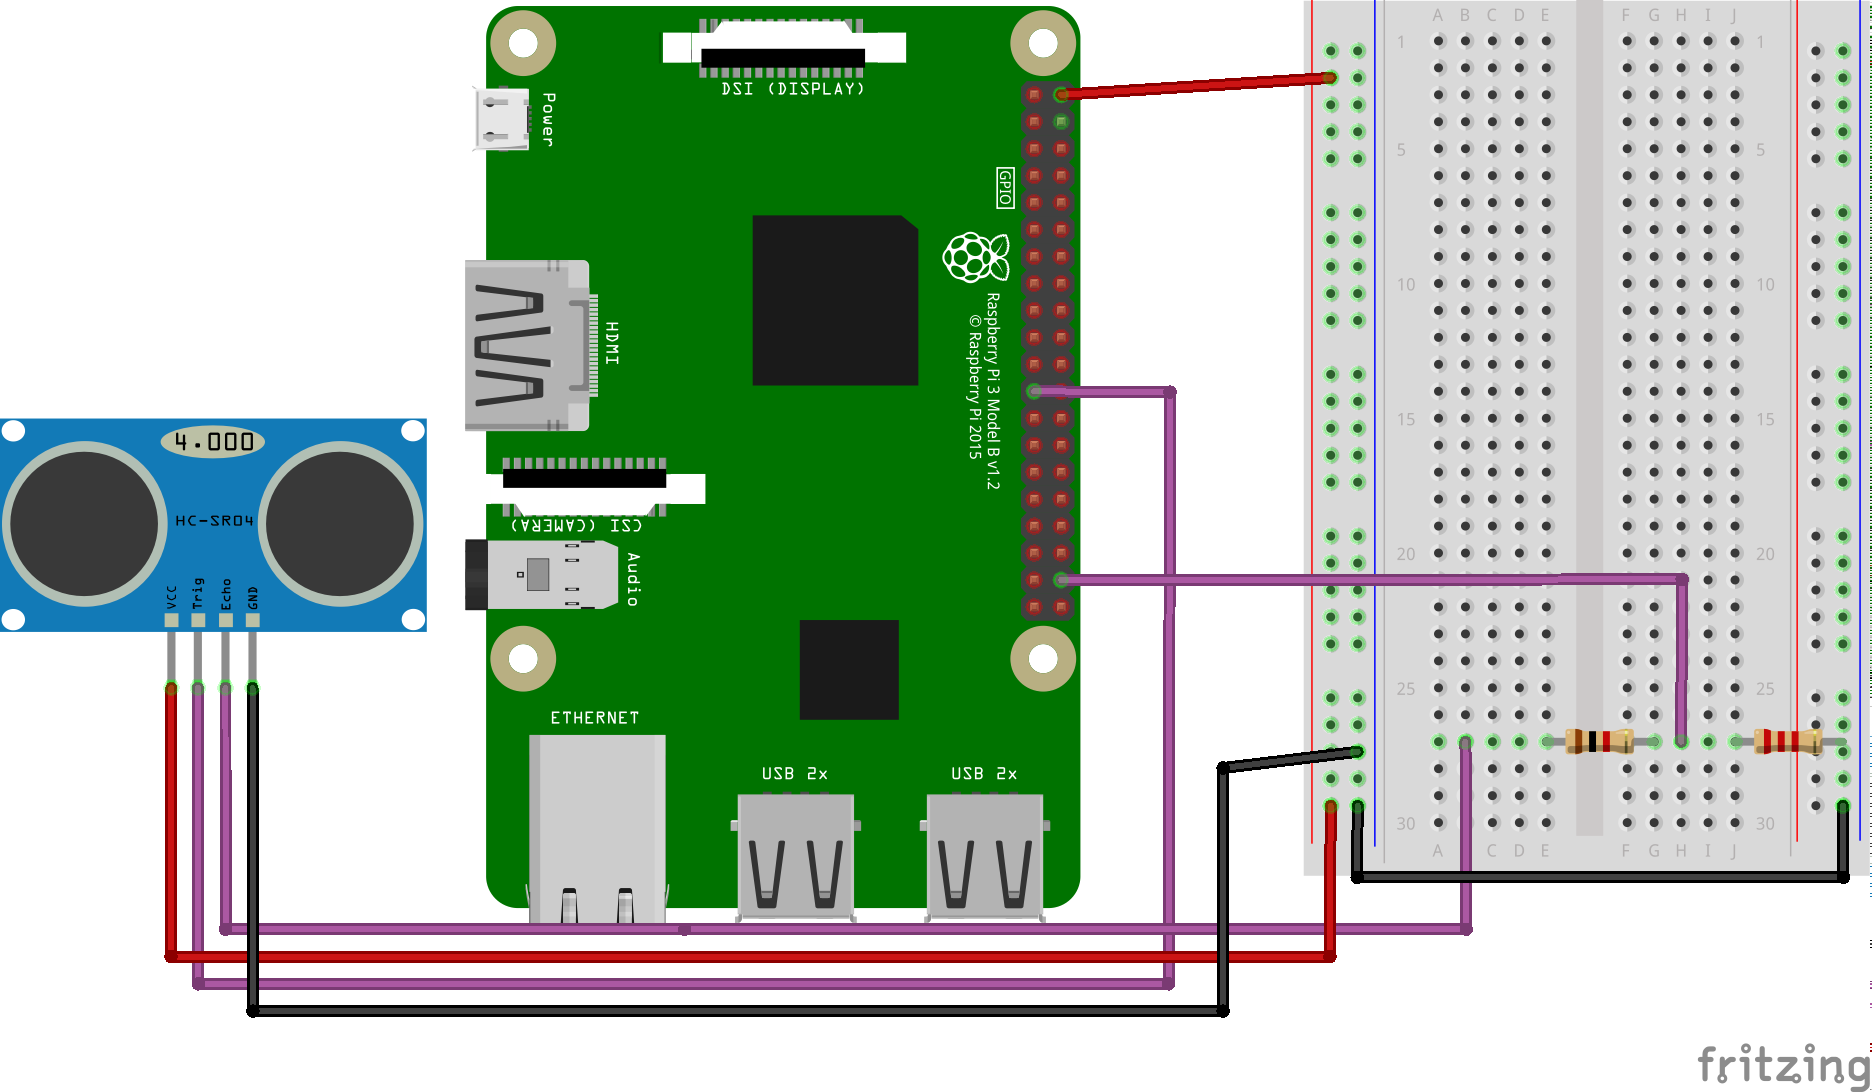
\includegraphics[width=0.5\textwidth]{images/smartGarage_Distance_bb.png}
\caption{Priklop HC-SR04 unltrazvočnega senzorja razdalje}
\end{figure}
\newpage
Da pridobim razdaljo, uporabim naslednjo metodo:
\begin{minted}[mathescape,
               linenos,
               numbersep=5pt,
               gobble=0,
               frame=lines,
               framesep=2mm]{python}
def checkCar():
    GPIO.output(GPIO_VARS_DICT['TRIG'], False)
    time.sleep(0.001)

    GPIO.output(GPIO_VARS_DICT['TRIG'], True)
    time.sleep(0.00001)
    GPIO.output(GPIO_VARS_DICT['TRIG'], False)

    while GPIO.input(GPIO_VARS_DICT['ECHO'])==0:
      pulse_start = time.time()

    while GPIO.input(GPIO_VARS_DICT['ECHO'])==1:
      pulse_end = time.time()

    pulse_duration = pulse_end - pulse_start
    distance = pulse_duration * 17150

    return round(distance, 2)
\end{minted}
\subsection{DS18B20 temperaturni senzor}
Ker sem v projektu prvič uporabil DS18B20 senzor temperature, sem si pomagal z vodičem na PiMyLifeUp \cite{PiMyLifeUp_DS18B20}.

Priklop je povsem enostaven. Vse kar potrebujemo, je DS18B20 senzor temperature in pa 4.7\SI{4.7}{\kohm} upor. Vcc nogico senzorja sem povezal na 3.3 V. GND nogico na GND, DATA nogico pa na BCM pin 19. Upor namestim med 3.3 V in DATA nogico senzorja.
\begin{figure}[h]
\centering
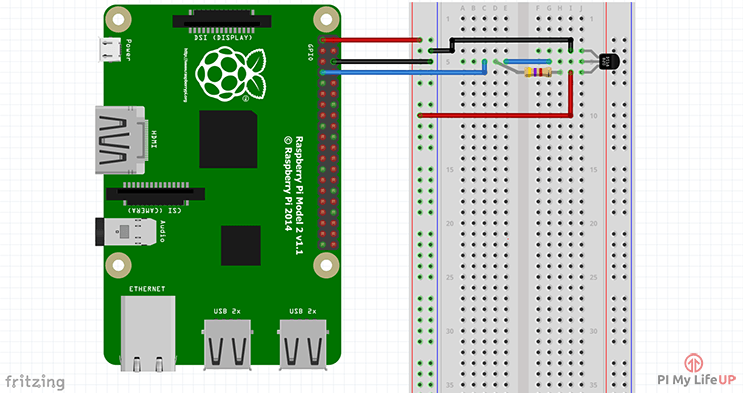
\includegraphics[width=0.5\textwidth]{images/DS18B20_diagram.png}
\source{Priklop DS18B20}{https://cdn.pimylifeup.com/wp-content/uploads/2016/03/Raspberry-Pi-Temperature-Sensor-Diagram-v2.png}
\end{figure}

\subsection{LCD zaslon}
Tudi priklop \gls{lcd} zaslona je bil zame nekaj novega. Zato sem si pomagal z vodičem na circuitbasics.com \cite{CB_LCD}.
Za priklop sem potreboval:
\begin{itemize}
    \item \gls{lcd} zaslon,
    \item 2 \SI{10}{\kohm} potenciometra.
\end{itemize}
\gls{lcd} zaslon sem priklopil na Raspberry Pi, kot je prikazano na spodnji sliki.
\begin{figure}[h]
\centering
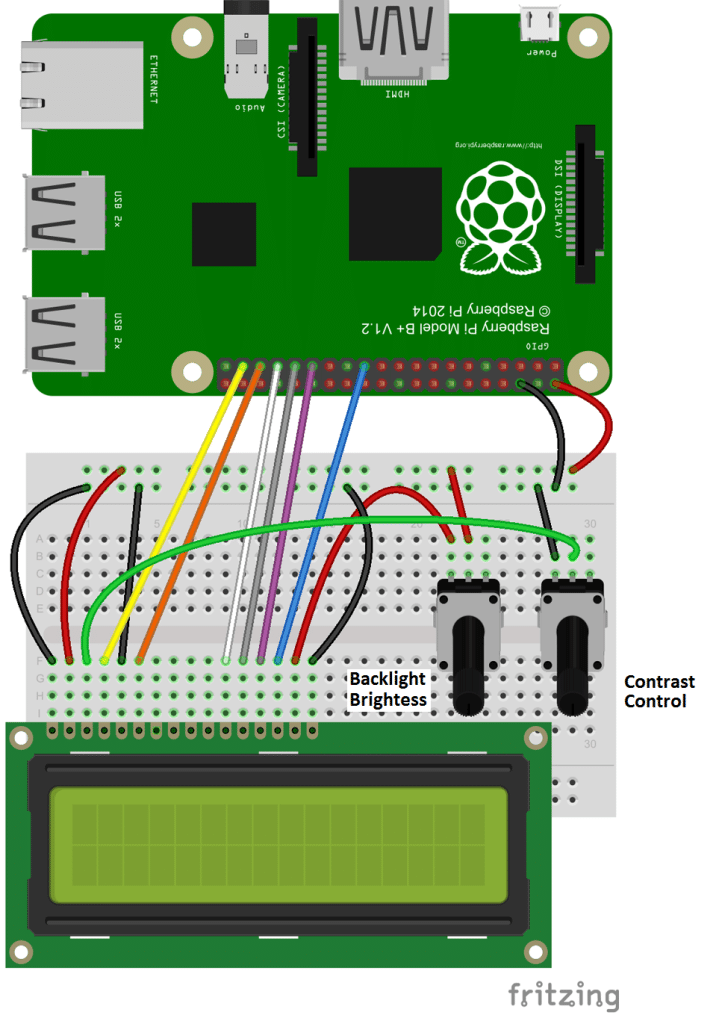
\includegraphics[width=0.3\textwidth]{images/LCD_4bit.png}
\source{Priklop LCD zaslona}{http://www.circuitbasics.com/wp-content/uploads/2015/04/Raspberry-Pi-LCD-4-bit-mode-719x1024.png}
\end{figure}
\newpage
\subsection{Tipki in LED diodi}
Priklop tipk in LED diod je zelo enostaven. Tipki povežem preko 3.3 V na poljuben \gls{gpio} pin, pri čemur pazim le, da je pin nastavljen kot vhodni in da je omogočen notranji pull down upor.
LED diodi sem priklopil preko \SI{270}{\ohm} uporov iz poljubnega \gls{gpio} pina na GND. \gls{gpio} pin mora biti nastavljen kot izhodni.
\begin{figure}[h]
\centering
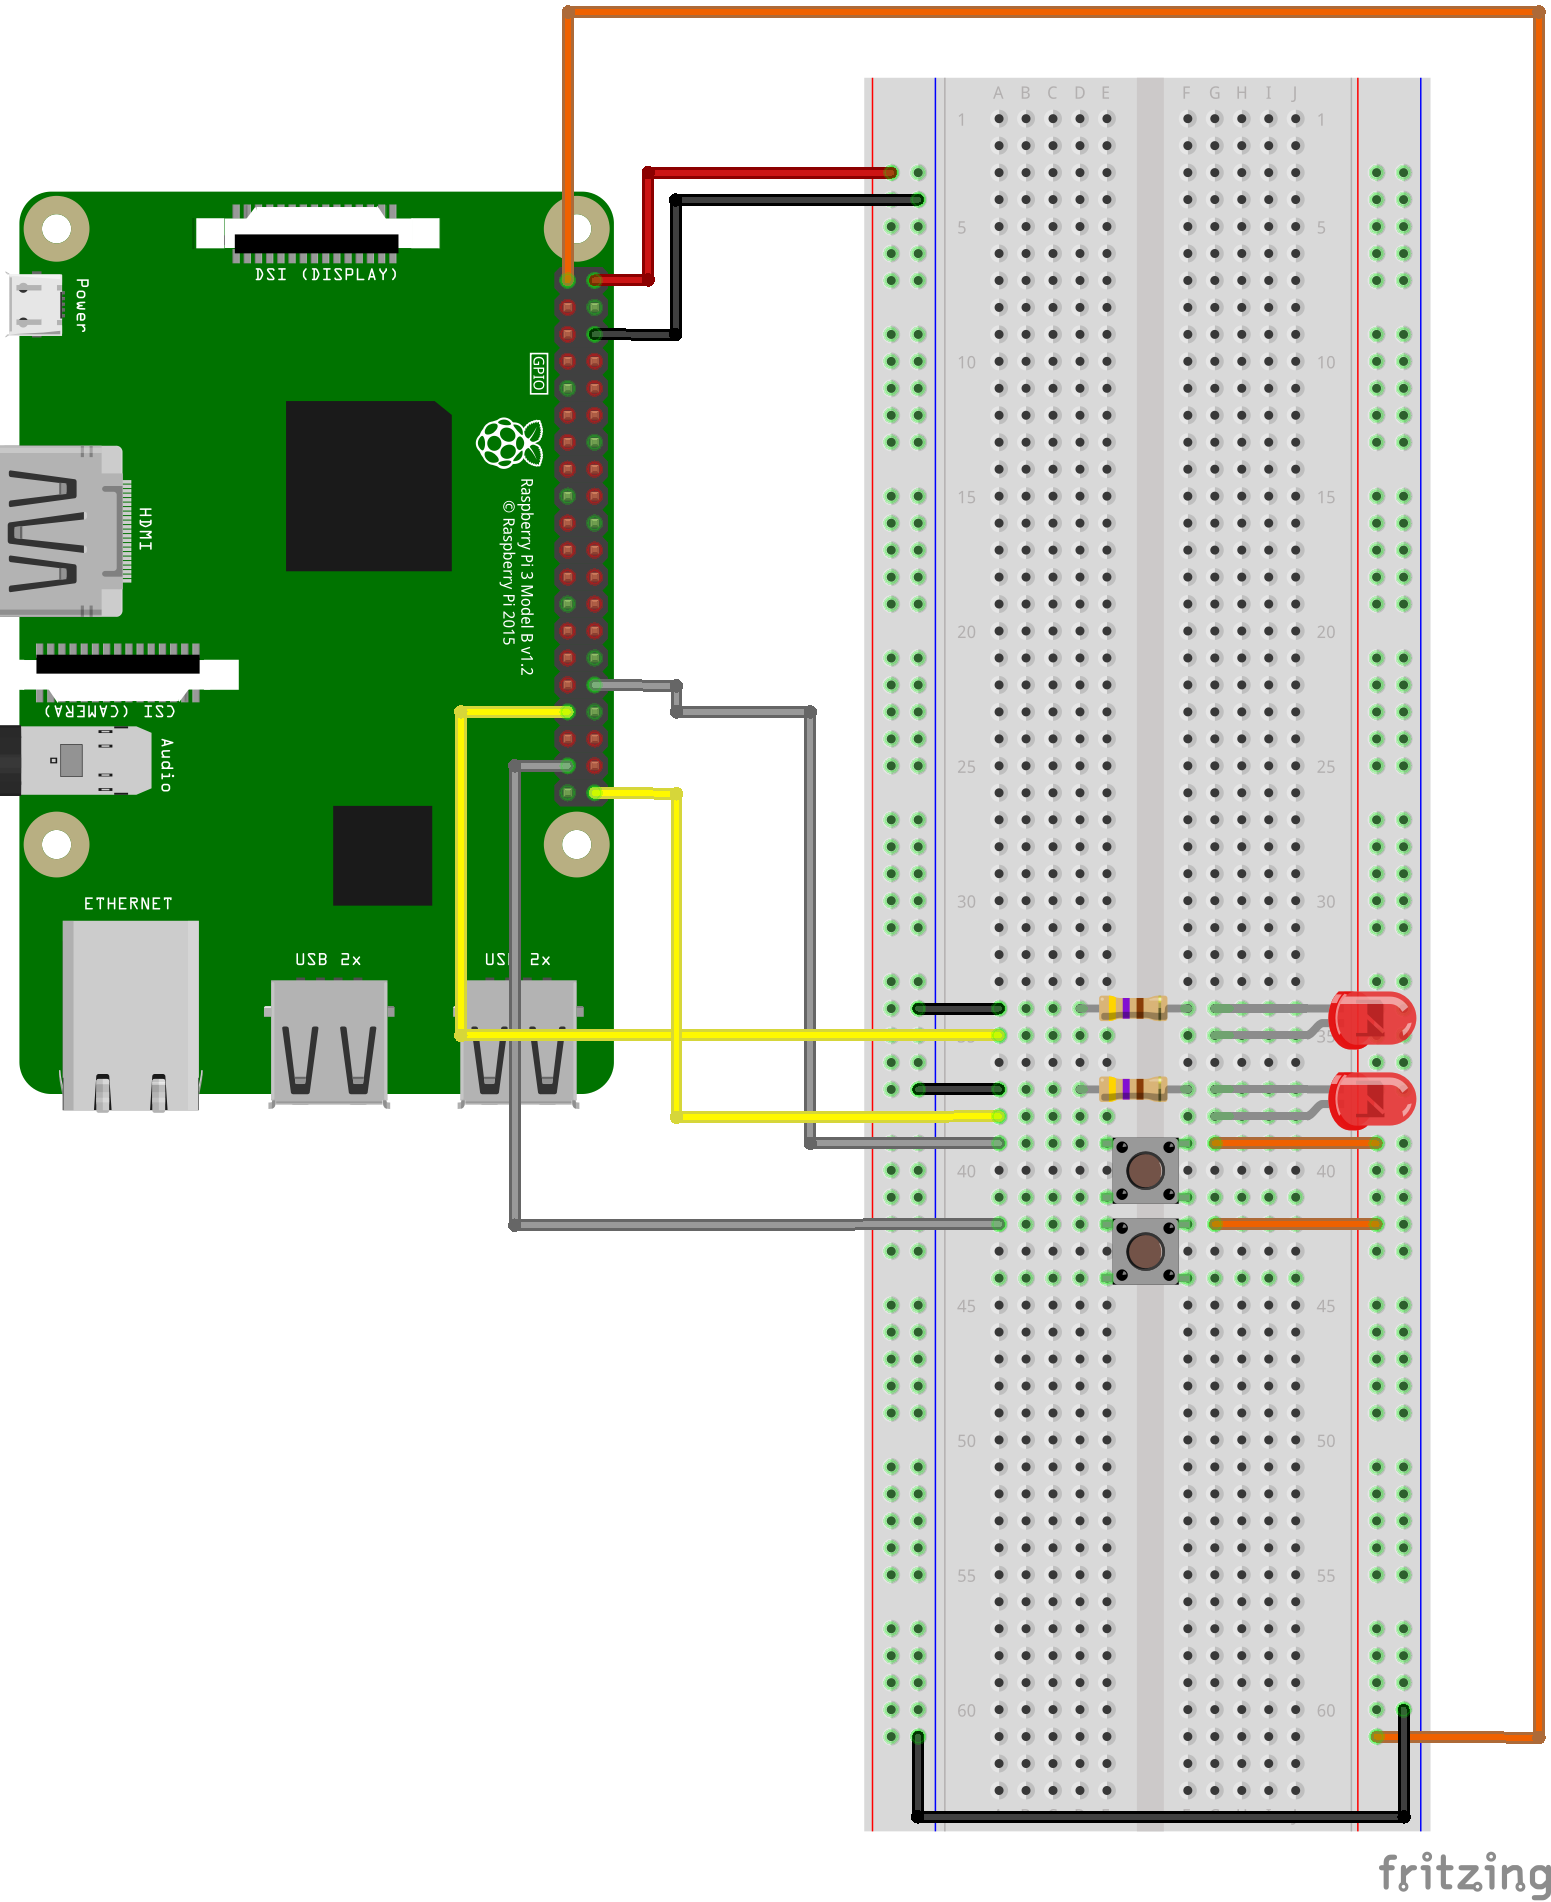
\includegraphics[width=0.4\textwidth]{images/smartGarage_LED_button_bb.png}
\caption{Priklop LED diod in tipk}
\end{figure}

\subsection{Vse komponente}
Ko sem priključil vsako komponento posebej in se prepričal o tem kako deluje, sem vse skupaj združil v en sistem.
\begin{figure}[h]
\centering
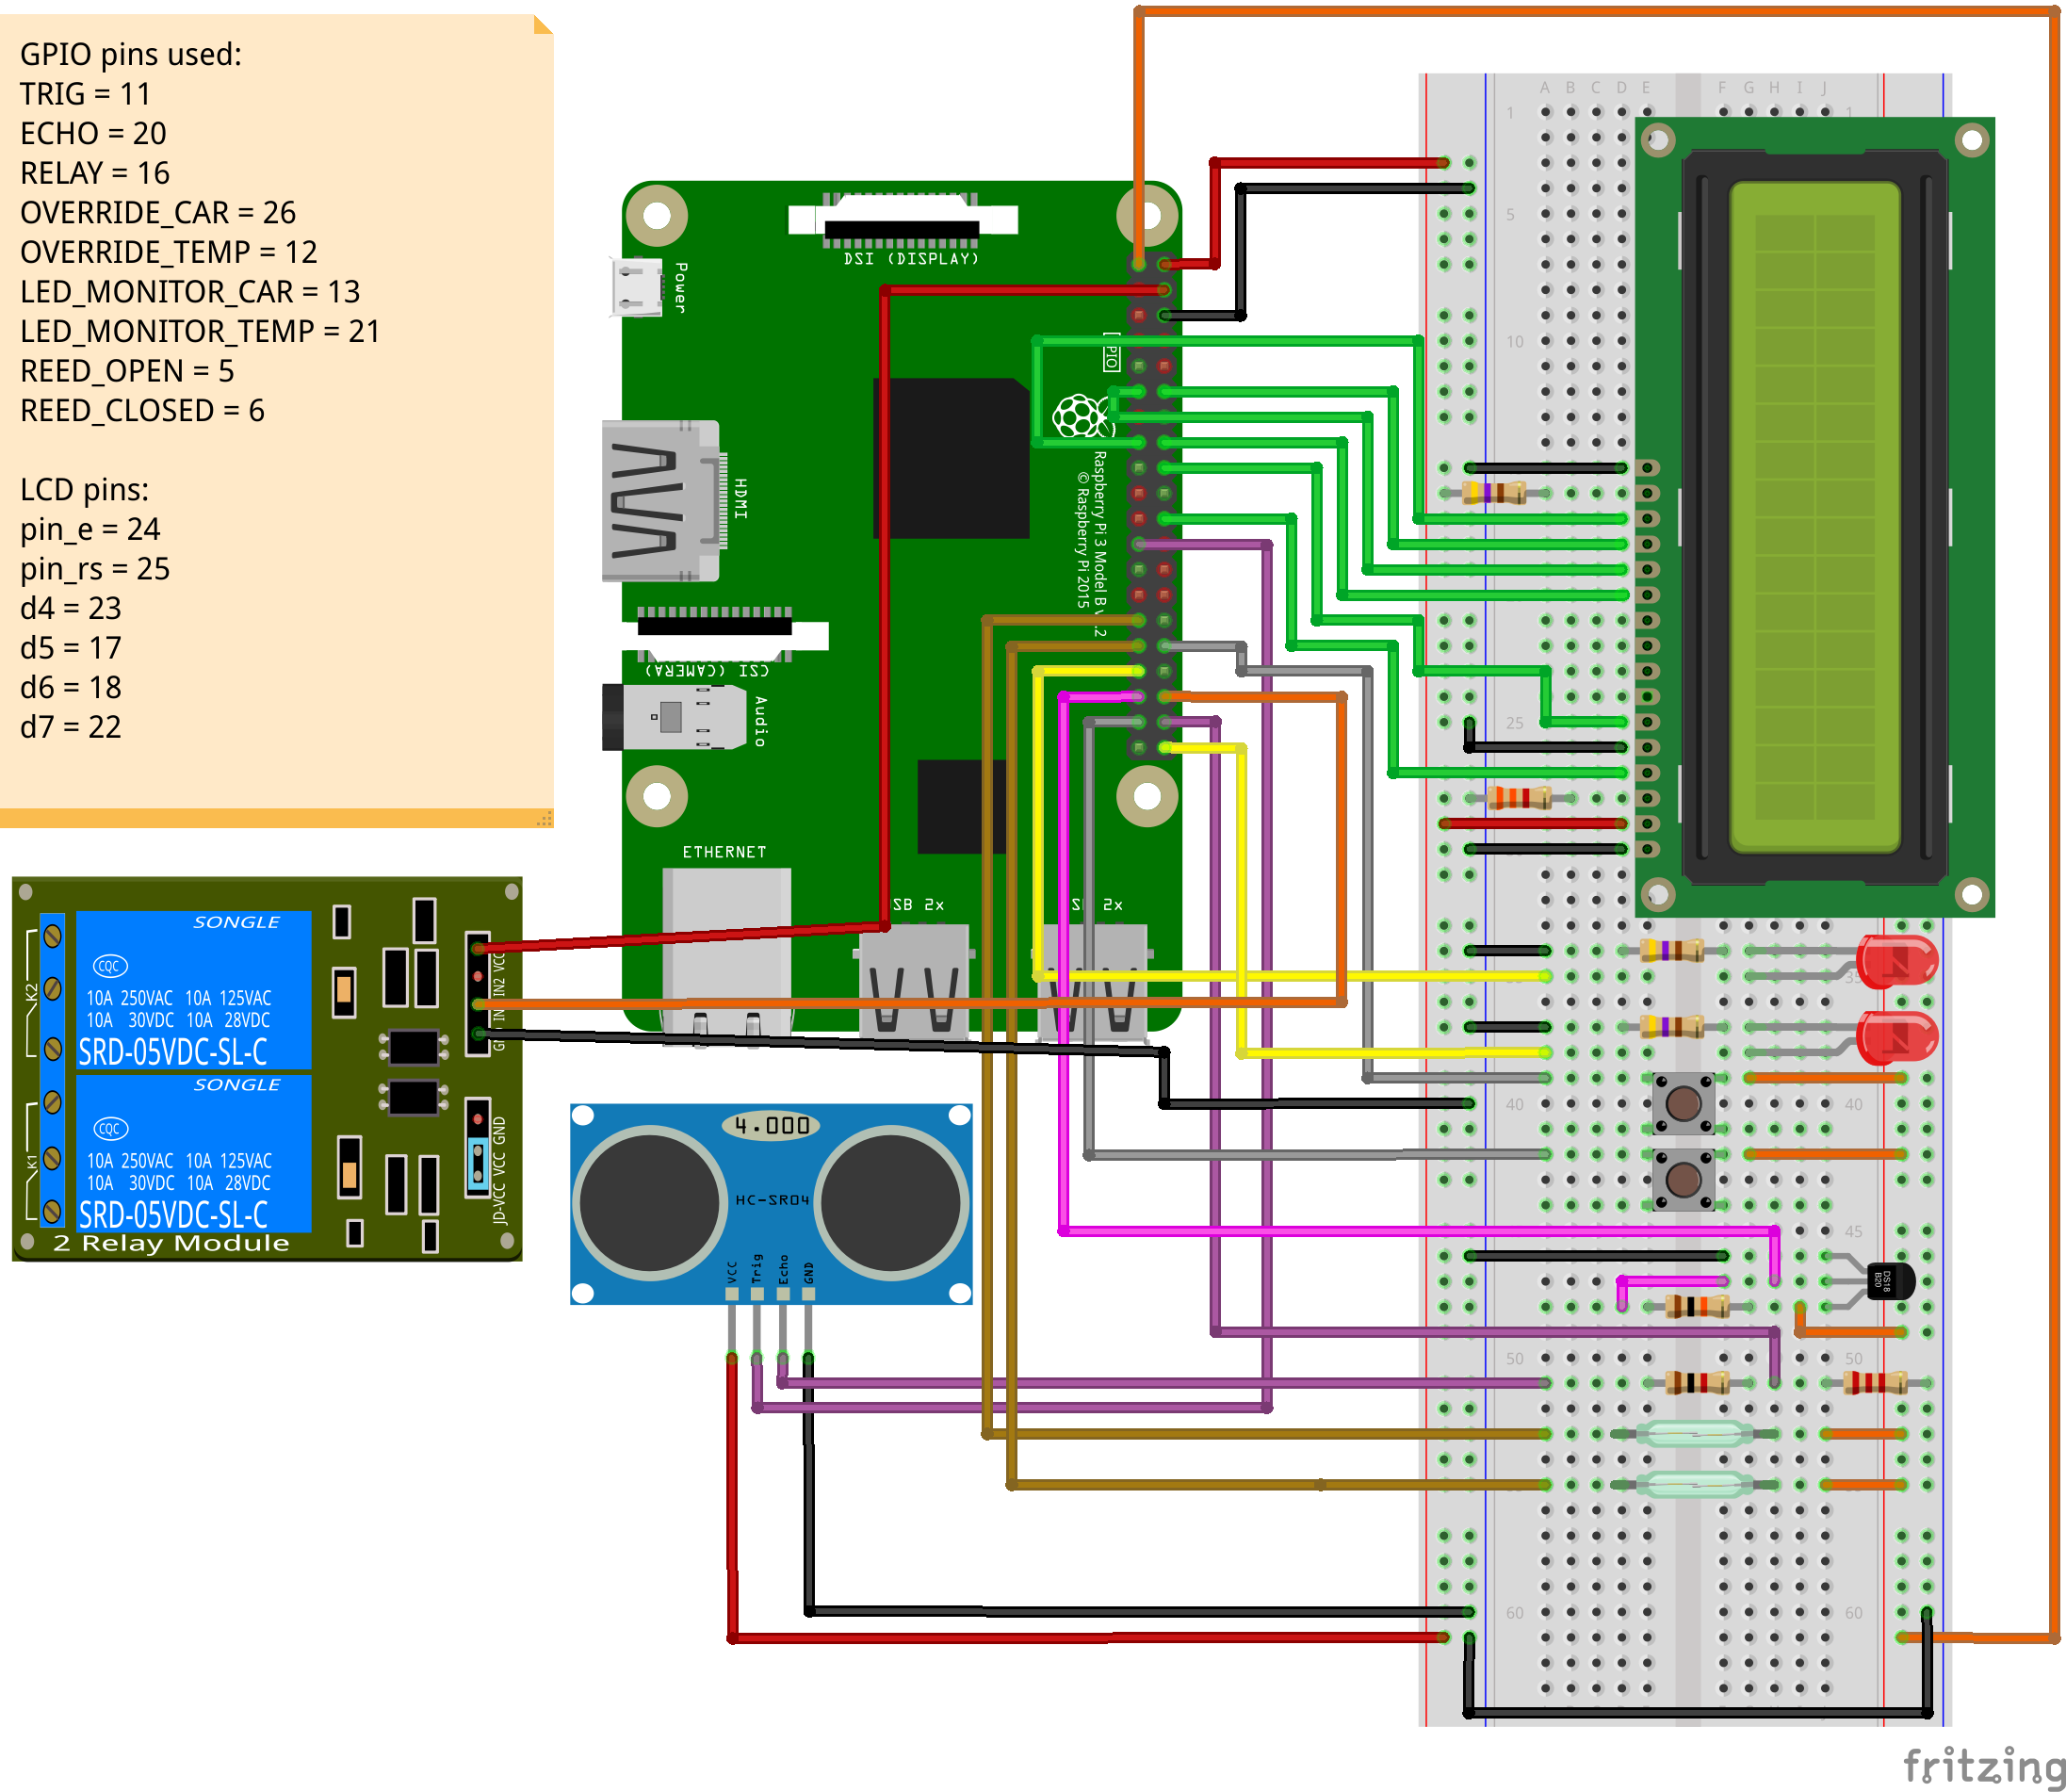
\includegraphics[width=0.5\textwidth]{images/smartGarageComplete_bb.png}
\caption{Priklop vseh komponent}
\end{figure}\\
Diagram se od dejanske izvedbe razlikuje le v tem da je tukaj uporabljen dvo kanalni modul relejev, ker je bil edini primeren za uporabo v diagramu. Ne glede na to je priklopljen samo en kanal.

\section{Programske rešitve}
Celotna koda vseh programov, omenjenih v raziskovalni nalogi, je v prilogi.
\subsection{Premikanje garažnih vrat}
Premikanje garažnih vrat je zelo enostavno. Vse, kar mora program storiti, da odpre garažna vrata, je preklop releja. Rele se tako preklopi iz odprtega stanja v zaprto, nato pa se čez pol sekunde vrne v odprto stanje. Za to poskrbi spodnja metoda.
\begin{minted}[mathescape,
               linenos,
               numbersep=5pt,
               gobble=0,
               frame=lines,
               framesep=2mm]{python}

def toggleGarage():
    GPIO.output(GPIO_VARS_DICT['RELAY'], 0)
    time.sleep(.5)
    GPIO.output(GPIO_VARS_DICT['RELAY'], 1)
\end{minted}
\subsection{Preveranje stanja garažnih vrat}
Preverjanje stanja garažnih vrat poteka z uporabo dveh reed stikal. Eno je nameščeno na spodnjem delu vodila garažnih vrat, kjer se vrata nahajajo ko so zaprta, drugo pa je nameščeno na zgornjem delu nosilca, kjer se vrata nahajajo, ko so odprta. Magnet, ki sproži stikali, je nameščen neposredno na garažna vrata.

Določanje, ali so vrata odprta, zaprta ali priprta, poteka s preverjanjem stanja stikal. Če je aktivno spodnje stikalo, pomeni, da so garažna vrata zaprta. Če je aktivno zgornje stikalo, pomeni, da so vrata odprta. Če ni aktivno nobeno izmed stikal, so garažna vrata priprta.

\subsection{Spremljanje temperature}
Spremljanje temperature poteka z uporabo DS18B20 temperaturnega senzorja. Ta je nameščen meter od tal na najmanj prepišnem delu garaže. Program začne spremljati temperaturo, ko se garažna vrata odprejo. Med spremljanjem temperature urtipa kontrolna LED dioda. Tako uporabnik ve, da program spremlja temperaturo v garaži. Če temperatura pade oziroma preseže nastavljeno mejo, program samodejno zapre vrata in o tem obvesti uporabnike. V primeru, da uporabnik ne želi, da program v primeru neprimerne temperature samodejno zapre vrata , lahko to prekliče s pritiskom tipke.

\subsection{Izpisovanje temperature na LCD}
\gls{lcd}, ki bo nameščen v ohišju na vidnem mestu v garaži, bo uporabljen za izpisovanje trenutega datuma, časa in temperature.

Za izpisovanje se uporablja poseben program, ki v neskončni zanki meri temperaturo ter jo skupaj s trenutnim datumem in časom izpisuje na \gls{lcd} zaslon.

\begin{figure}[h]
\centering
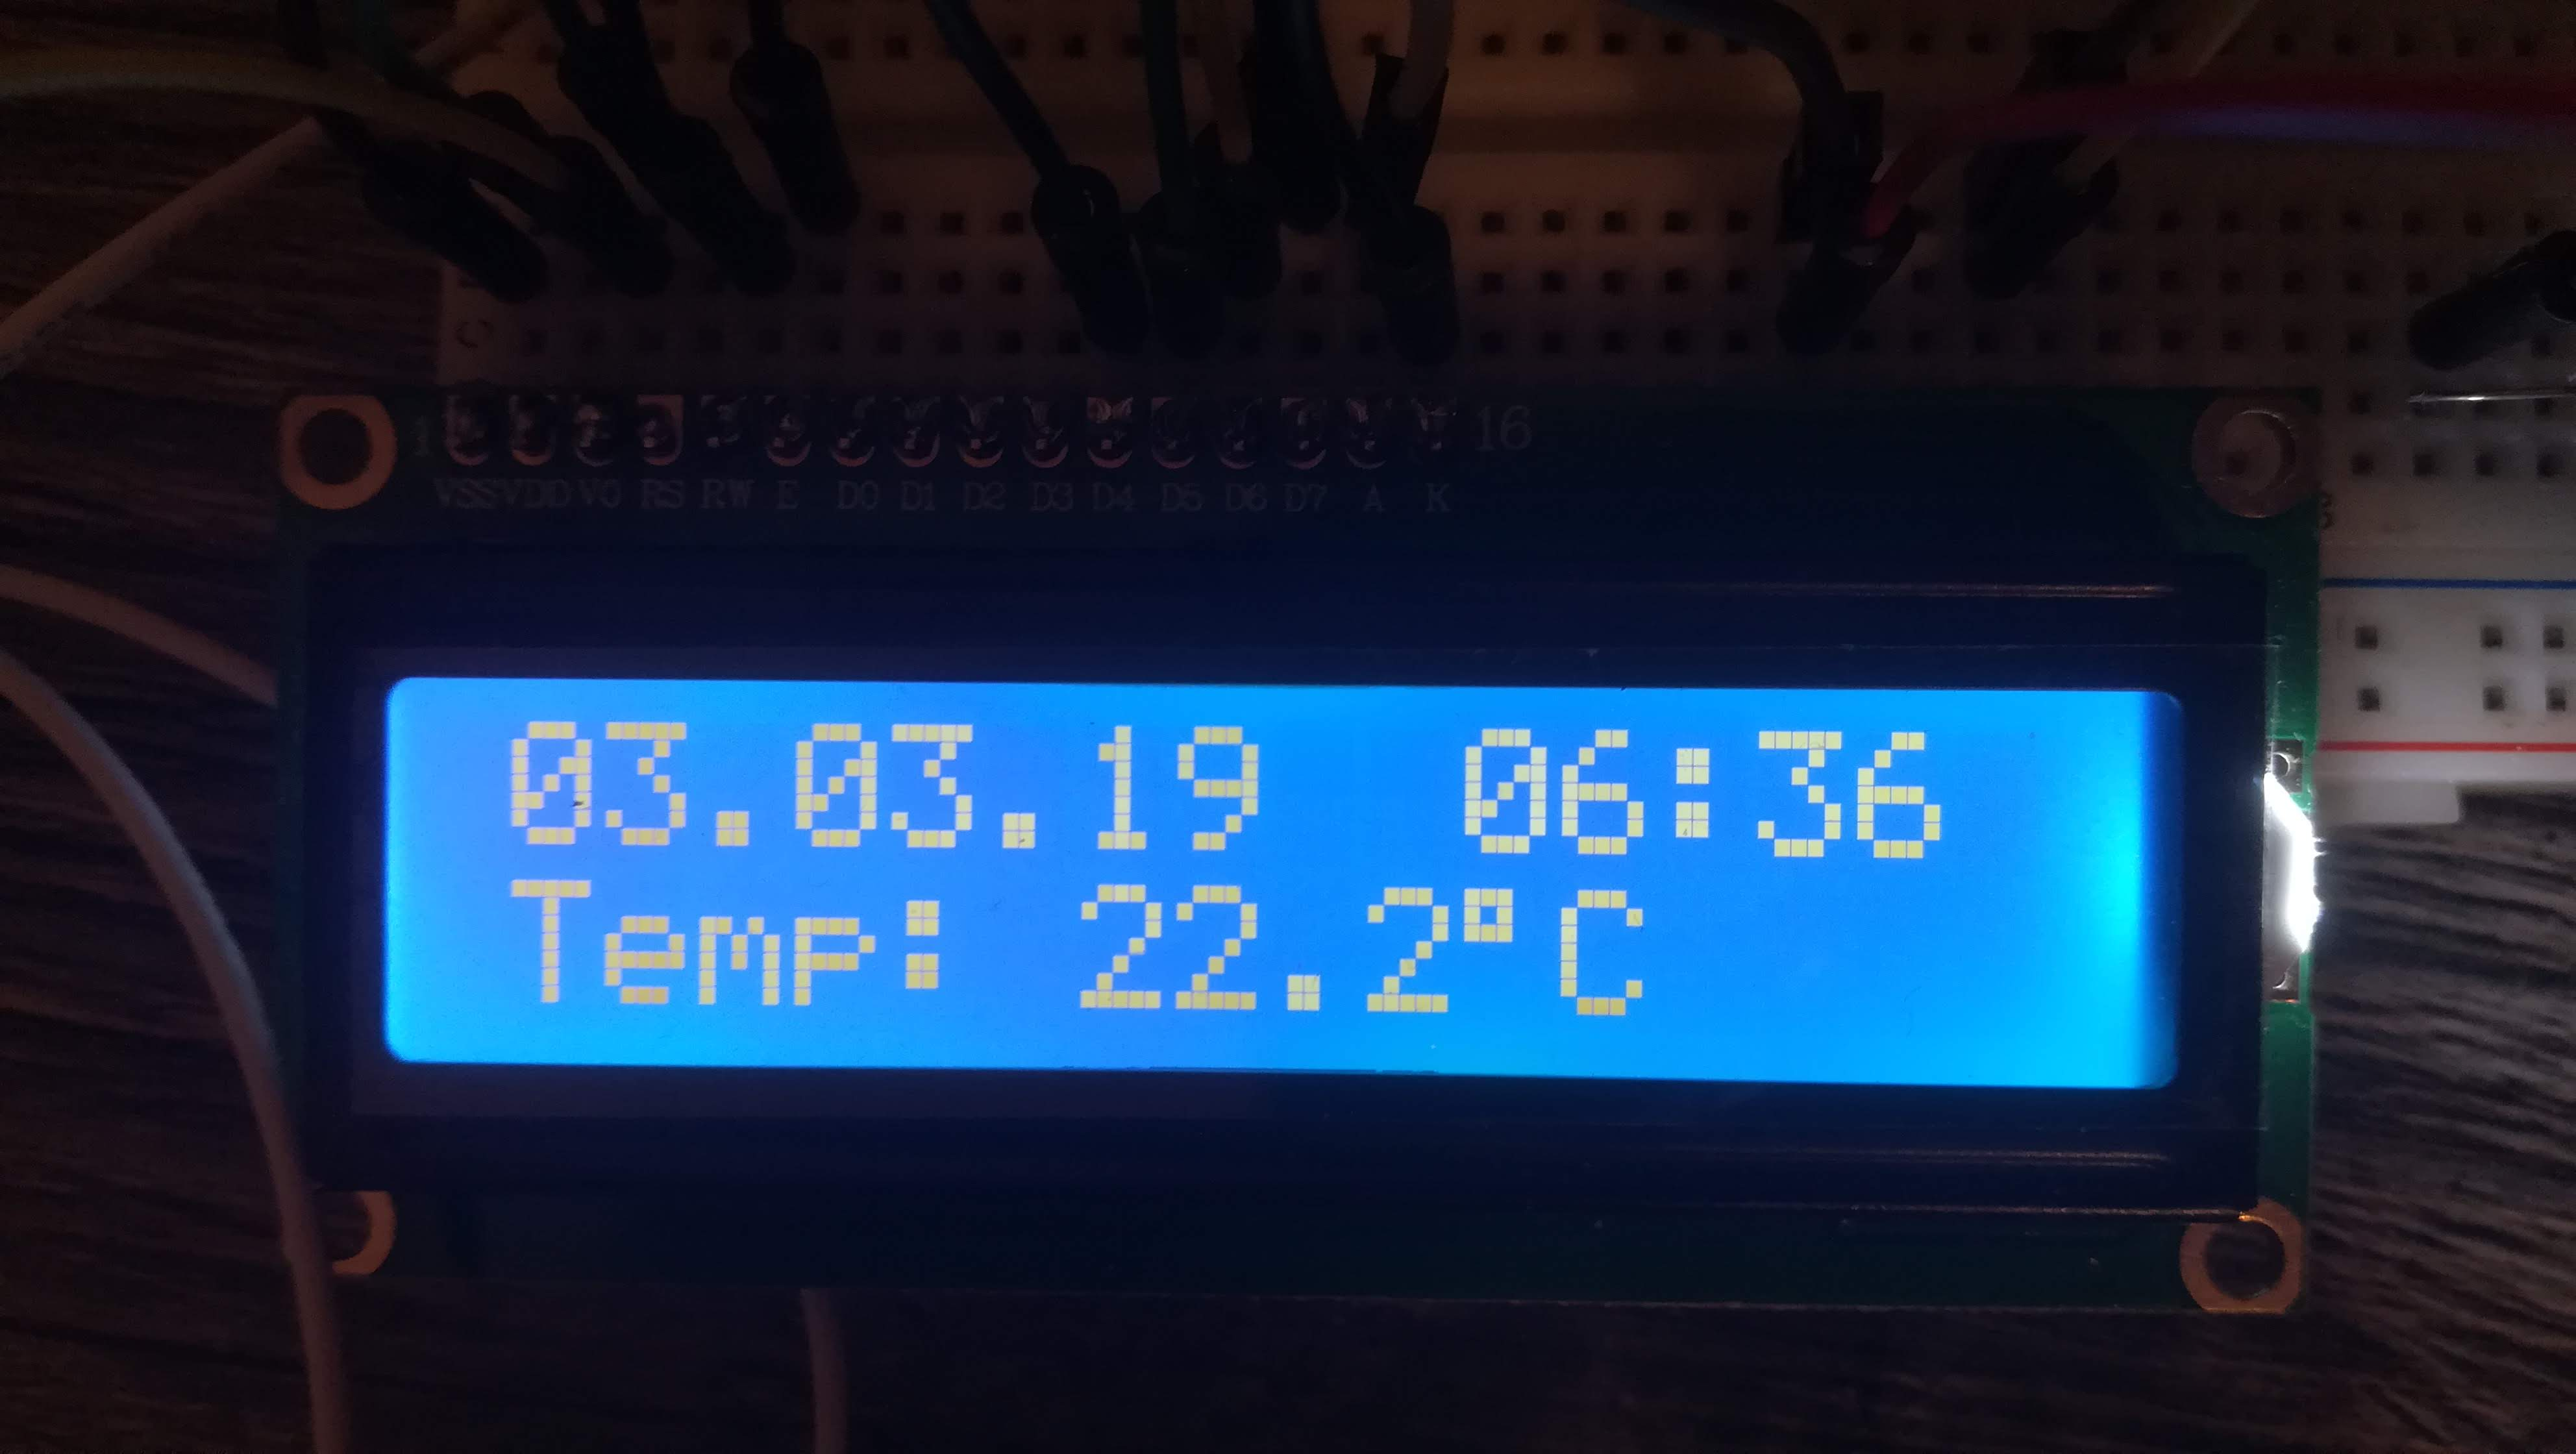
\includegraphics[width=0.5\textwidth]{images/LCD_temp.jpg}
\caption{Izpis na LCD}
\end{figure}

\subsection{Samodejno zapiranje glede na avto}
Ultrazvočni senzor razdalje HC-SR04 se uporablja za preverjanje, ali je avto v garaži ali ne. Če na primer avta ni v garaži, nato pa se garaža odpre in vanjo pripelje avto, bo program po določenem času samodejno zaprl vrata in o tem obvestil uporabnike preko potisnih sporočil. Enako se zgodi, če avto zapusti garažo. V primeru, da uporabnik ne želi, da se ob prihodu ali odhodu avta iz garaže vrata samodejno zaprejo, lahko ukaz prekliče s pritiskom tipke.

Senzor je nameščen na stropu garaže. Razdalja (med senzorjem in avtom), ki določa, kdaj senzor zazna, da je v garaži avto, se nastavi v konfiguracijski datoteki.

\subsection{Če garažnih vrat ni možno zapreti}
Med testiranjem programa za garažna vrata sem kmalu odkril relativno pomembno napako. Dogajalo se je, da je program želel vrata zapreti, to pa zaradi npr. ovire pod vrati ni bilo mogoče. Ker program ni bil dobro napisan, je v nedogled poskušal brez uspeha zapreti vrata.

Težavo sem rešil tako, da sem napisal metodo v katero program vstopi, če se vrata po poskusu zapiranja ne zaprejo. Metoda nato še nekajkrat poskuša zapreti vrata. Če to ni mogoče, vrata ostanejo priprta.

\begin{minted}[mathescape,
               linenos,
               numbersep=5pt,
               gobble=0,
               frame=lines,
               breaklines=true,
               framesep=2mm]{python}

def doorAjar():
    for attempts in range(0, TIMEOUTS_VARS_DICT['AJAR_CLOSE_ATTEMPTS']):
        toggleGarage()
        for x in range(0, TIMEOUTS_VARS_DICT['AJAR_TIMEOUT']):
            if checkDoor() != 'priprta':
                break
            time.sleep(1)
        if checkDoor() == 'zaprta':
            break
\end{minted}

\subsection{Konfiguracijska datoteka}
Za lažje nastavljanje spremenljivk, kot je na primer termperatura, pri kateri se garažna vrata zaprejo, sem se odločil uporabiti konifugacijsko datoteko.

Ker te do sedaj še nikoli nisem uporabljal, mi je bila uradna Pythonova dokumentacija \cite{Py_configParser} v veliko pomoč.

\subsubsection{Datoteka}
Zgradba konfiguracijske datoteke je zelo preprosta. V oglatih oklepajih se nahaja ime odseka, sledijo imena spremenljivk, katerih vrednost je določena z enačajem, ki mu sledi vrednost.
\begin{minted}[mathescape,
               linenos,
               numbersep=5pt,
               gobble=0,
               frame=lines,
               breaklines=true,
               framesep=2mm]{python}

[gpio]
TRIG = 11
ECHO = 20
RELAY = 16
\end{minted}

\subsubsection{Branje iz datoteke}
Branje iz datoteke je bilo na začetku kar precejšen izziv. Po nekaj različnih poskusih implementacije sem se določil da bom vrednosti iz konfiguracijske datoteke shranjeval v slovar. Za branje iz datoteke sem napisal svojo metodo.

Ta prejme del, iz katerega mora brati, spremenljivke, ki jih je potrebo prebrati in slovar v katerega se bodo shranile vrednosti. Nato odpre datoteko za branje, nato pa v zanki prebere vrednosti spremenljivk in jih shrani v slovar.

\subsection{Potisna obvestila}
Ker je potrebno uporabnike obveščati o spremebi stanja garažnih vrat, sem moral poiskati način, kako to storiti. S pomočjo raziskovanja sem se odločil, da bom uporabil storitev za pošiljanje potisnih obvestil Pushover \cite{Pushover}.

Storitev je zelo enostavna in se je do sedaj odlično obnesla. Edina slabost je, da je plačljiva. Treba je namreč kupiti licenco za vsako napravo, ki storitev uporablja. Cena licence je 4.99 \$.
\subsection{Možne razširitve projekta}
Čeprav sem s projektom do sedaj zelo zadovoljen, sem prepričan, da je možnosti za izboljšave še veliko.
\subsubsection{Sistem dnevniških datotek}
Beleženje dogodkov programa je dobro že z vidika odpravljanja težav. Trenutno je zelo težko določiti, kje v programu se pojavlja napaka. Zato bi bilo zelo koristno, če bi v program dodal zapisovanje dnevniški datotek in pa možnost razhroščevanja programa (debug).

Druga stvar, ki bi bila po mojem mnenju koristna, pa je beleženje kdo je garažo aktiviral, kdaj in s katere naprave. Iz tega bi lahko delal statistiko uporabe garažnih vrat, hkrati pa bi lahko zelo hitro ugotovil, če do garaže dostopa kdo, ki nima pooblastil.
\subsubsection{Android aplikacija}
Trenutno za upravljanje garaže preko telefona uporabljam kar Shell skripto, ki jo poženem z aplikacijo Termux. Zaradi boljše uporabniške izkušnje in uporabnosti bi bilo zato zelo dobro, če bi naredil še aplikacijo za Android. Aplikacija bi se lahko uporabljala za upravljanje garažnih vrat in spremljanje temperature. Lahko bi dodal tudi možnost, da uporabniki preko aplikacije nastavijo določene spremenljivke, kot je na primer ura, ob kateri se garaža samodejno zapre.
\subsubsection{Brezžični moduli}
Ko sem razmišljal, kako bi lahko svoj projekt še dodatno izboljšal, sem prišel na idejo, da bi bili moduli samostojni. Tako bi bil na primer en modul rele, drugi bi bil \gls{lcd} zaslon, tretji senzor temperature itd.
To bi bilo verjetno izvedljivo, če bi za vsak modul uporabil na primer NodeMcu \cite{NodeMcu}. Tako bi bil vsak modul zase povezan v WiFi omrežje, preko katerega bi komuniciral s centralnim računalnikom.

\subsubsection{Odpiranje s prstnim odtisom ali številčnico}
Kaj storiti v primeru, če želimo od zunaj odpreti garažo a pri sebi nimamo ne daljinca ne pametnega telefona? To težavo bi lahko enostavno rešili tako, da bi na zunanji strani vrat namestili čitalec prstnih odtisov ali številčnico. Tako bi lahko uporabniki odprli garažna vrata s prstnim odtisom ali z ustrezno kodo.

\subsubsection{Spletna stran}
Za spremljanje stanja garažnih vrat in njihovo upravljanje bi bilo dobro imeti tudi spletno stran. Poleg tega bi se lahko slednja uporabila (če bi se prijavil ustrezen uporabnik) za spremljanje dnevniških datotek in nastavljenje določenih parametrov programa.
\newpage

\section{Razprava}
\begin{comment}
Moje hipoteze so bile:
\begin{enumerate}
  \setlength\itemsep{0.5mm}
    \item Garažna vrata bo možno upravljati preko telefona
    \item Garažna vrata bo možno upravljati preko spletne strani
    \item Raspberry Pi bo spremljal ali je avto v garaži ali ne in glede na to samodejno zapiral garažna vrata
    \item Raspberry Pi bo spremljal temperaturo v garaži in jih samodejno zaprl v primeru prenizke ali previsoke temperature
    \item Raspberry Pi bo samodejno zaprl garažna vrata, če ostanejo odprta po določeni uri
    \item Raspberry Pi nas bo preko potisnih obvestil obveščal o spremembi stanja garažnih vrat
    \item Raspberry Pi bo beležil kdo in kdaj je aktiviral garažna vrata
    \item uporabnik bo imel možnost preklicati samodejno zapiranje vrat
\end{enumerate}

\vspace{5mm}
\end{comment}
\begin{enumerate}
  %\setlength\itemsep{0.5mm}
  \item Prvo hipotezo: garažna vrata bo možno upravljati preko telefona, lahko delno potrdim, saj je uporavljanje vrat s telefonom možno, vendar le, če so na njem nameščene ustrezne aplikacije (Termux ali PiRelay).
  \item Drugo hipotezo: garažna vrata bo možno upravljati preko spletne strani, ovržem, saj mi spletne strani ni uspelo narediti.
  \item Tretjo hipotezo: Raspberry Pi bo spremljal ali je avto v garaži ali ne in glede na to samodejno zapiral garažna vrata, lahko potrdim, saj se garažna vrata samodejno zaprejo, če avto pripelje v garažo ali jo zapusti.
  \item Tudi četrto hipotezo: Raspberry Pi bo spremljal temperaturo v garaži in jih samodejno zaprl v primeru prenizke ali previsoke temperature, lahko potrdim, saj se garaža ob neprimerni temperaturi samodejno zapre.
  \item Peto hipotezo: Raspberry Pi nas bo preko potisnih obvestil obveščal o spremembi stanja garažnih vrat, lahko potrdim, saj Raspberry Pi pošilja potisna obvestila preko soritve Pushover.
  \item Šesto hipotezo: Raspberry Pi bo beležil kdo in kdaj je aktiviral garažna vrata, ovržem, saj Raspberry Pi ne beleži dnevnika uporabe garaže.
  \item Sedmo hipotezo: uporabnik bo imel možnost preklicati samodejno zapiranje vrat, lahko delno potrdim. Uporabnik ima možnost preklicati samodejno zapiranje vrat v primeru neustrezne temperature ali spremembe stanja avta. Ne more pa preklicati samodejnega zapiranja ob določeni uri.
\end{enumerate}
\subsection{Težave med delom}
\subsubsection{Rele predolgo ostane zaprt}
Prva težava, ki se je pojavila pri izdelavi mojega projekta, je bilo, da je rele ostal predolgo zaprt. To je pomenilo, da se je rele zaprl, garažna vrataso se začela premikati, nato pa se ni več odprl. Ko se je to zgodilo, garažnih vrat ni bilo mogoče uporavljati s tipko.

Težavo sem rešil zelo preprosto. Napisal sem program (checkRelay.py), ki spremlja stanje releja.V priemru, da ta ostane zaprt predolgo, ga odpre, dogodek ap zabeleži v dnevniško datoteko (checkRelay.log).

\subsubsection{Multithreading}
Med izdelavo projekta sem se kmalu zavedel, da imam še eno težavo. Program mora hkrati spremljati temperaturo v garaži in stanje avta. Najprej sem razmišljal, da bom problem rešil z uporabo Multithreadinga. Tako sem prebral vodič \cite{tutorialspoint_MT}. Ker po nekaj neuspešnih poskusih še vedno nisem vedel kaj natanko moram storiti, sem začel iskati alternative.

Na koncu mi je težavo uspelo rešiti z uporabo multiprocessinga. Najprej sem prebral dokumentacijo \cite{python_MP}, nato pa sem z nekaj eksperimentiranja težavo kmalu odpravil.

Izdelava raziskovalne naloge je zahtevala veliko truda in časa. Moral sem prebrati veliko dokumentacije, brskati po forumih, eksperimentirati. :e bi imel več časa, denarja in še kakšen dodaten par rok, pa bi lahko svoj projekt še precej razširil.
\newpage
\section{Zaključek}
Moj cilj je bil narediti funkcionalen izdelek, ki se bo namestil v garaži in se uporabljal za avtomatizacijo garažnih vrat ter upravljanje le teh preko telefona. Čeprav nimam estetsko dovršenega in praktično uporabnega izdelka, pa imam delujoč prototip.

Med izdelavo raziskovalne naloge sem pridobil veliko novih znanj. Dobil sem tudi kar precej izkušenj pri delu z elektroniko, ki jih do sedaj nisem imel.

Projekt zame še zdaleč ni končan. Razvoj sistema bom nadaljeval kolikor bo čas dopuščal, seveda pa bom moral upoštevati tudi finančne omejitve. Odlično bi bilo tudi, če bi našel še koga, ki bi bil pripravljen sodelovati pri projektu. Kot vedno pravijo, več glav več ve.
%%--------------------------------Beginning of Acronyms & Glossary--------------------------------%%
\newpage
\clearpage

%%\printglossary[type=\acronymtype]

%\printglossary[type=main]
%%--------------------------------End of Acronyms & Glossary--------------------------------%%

%%--------------------------------Beginning of Bibliography--------------------------------%%
\begin{flushleft}
\bibliographystyle{plain}
\bibliography{sources.bib}
\end{flushleft}
%%--------------------------------End of Bibliography--------------------------------%%
\newpage
\section{Zahvale}
Zahvaljujem se svojemu mentorju, profesorju Borotu Slemenšku za nasvete ter pomoč pri izdelavi raziskovalne naloge.
\newpage
\section{Priloge}
\subsection{Izjava}
\begin{figure}[h]
\centering

\includegraphics[width=0.85\textwidth]{images/izjava.jpg}
\end{figure}
\newpage
\subsection{garage.py - glavni program}
\begin{minted}[mathescape,
               linenos,
               numbersep=5pt,
               gobble=0,
               frame=lines,
               breaklines=true,
               framesep=2mm]{python}

#!/usr/bin/python
# -*- coding: utf-8 -*-

import RPi.GPIO as GPIO
import time
import argparse
import os
import time
import glob
from RPLCD.gpio import CharLCD
from multiprocessing import Process
from pushover import Client
import ConfigParser
import io
import logging
from logging.config import fileConfig

#fileConfig('logging_config.ini')
#logger = logging.getLogger()

GPIO.setwarnings(False)

homeFolder=os.environ['HOME'] #pridobim domačo mapo uporabnika, ki je pognal program
logPath=homeFolder+'/.garage/logs' #nastavim mapo v katero se bo shranjevala dnevniška datoteka
logFile=homeFolder+'/.garage/logs/toggleRelay.log'

def checkLogFilePath(): #metoda, ki preveri ali obstajajo vse ptrebne mape in jih po potrebi ustvari
    if(not os.path.exists(homeFolder+'/.garage')):
        os.mkdir(homeFolder+'/.garage')
    if(not os.path.exists(logPath)):
        os.mkdir(logPath)

def readConf(section, vars, val_dict):
    configParser = ConfigParser.RawConfigParser(allow_no_value=True)
    configParser.read(os.environ['HOME']+'/.garage/garage.conf')
    for value in vars:
        val_dict[value] = int(configParser.get(section, value))

def lcd_write(line1, line2):
    lcd.clear()
    lcd.cursor_pos = (0, 0)
    lcd.write_string(line1)
    lcd.cursor_pos = (1, 0)
    lcd.write_string(line2)

def read_temp_raw():
    f = open(device_file, 'r')
    lines = f.readlines()
    f.close()
    return lines

def read_temp():
    lines = read_temp_raw()
    while lines[0].strip()[-3:] != 'YES':
        time.sleep(0.2)
        lines = read_temp_raw()
    equals_pos = lines[1].find('t=')
    if equals_pos != -1:
        temp_string = lines[1][equals_pos+2:]
        temp_c = int(temp_string) / 1000.0 # TEMP_STRING IS THE SENSOR OUTPUT, MAKE SURE IT'S AN INTEGER TO DO THE MATH
        temp_c = round(temp_c, 1) # ROUND THE RESULT TO 1 PLACE AFTER THE DECIMAL
        return temp_c

def blink(LED):
    GPIO.output(LED, GPIO.HIGH)  # led on
    time.sleep(.5)
    GPIO.output(LED, GPIO.LOW) # led off
    time.sleep(.5)

def toggleGarage():
    GPIO.output(GPIO_VARS_DICT['RELAY'], 0)
    time.sleep(.5)
    GPIO.output(GPIO_VARS_DICT['RELAY'], 1)

def checkDoor():
    if GPIO.input(GPIO_VARS_DICT['REED_OPEN']) == True:
        return "odprta"
    elif GPIO.input(GPIO_VARS_DICT['REED_CLOSED']) == True:
        return "zaprta"
    else:
        return "priprta"

def checkCar():
    GPIO.output(GPIO_VARS_DICT['TRIG'], False)
    time.sleep(0.001)

    GPIO.output(GPIO_VARS_DICT['TRIG'], True)
    time.sleep(0.00001)
    GPIO.output(GPIO_VARS_DICT['TRIG'], False)

    while GPIO.input(GPIO_VARS_DICT['ECHO'])==0:
      pulse_start = time.time()

    while GPIO.input(GPIO_VARS_DICT['ECHO'])==1:
      pulse_end = time.time()

    pulse_duration = pulse_end - pulse_start
    distance = pulse_duration * 17150

    return round(distance, 2)

def monitorCar():
    GPIO.add_event_detect(GPIO_VARS_DICT['OVERRIDE_CAR'],GPIO.RISING,bouncetime=300)
    distance = checkCar()
    for x in range(0,TIMEOUTS_VARS_DICT['CAR_STATUS_TIMEOUT']):
        if GPIO.event_detected(GPIO_VARS_DICT['OVERRIDE_CAR']):
            break
        elif checkDoor() == 'zaprta':
            break
        blink(GPIO_VARS_DICT['LED_MONITOR_CAR'])
        if (distance >=25 and checkCar() <= 20) or (distance <=20 and checkCar() >= 25):
            for i in range(0,5):
                blink(GPIO_VARS_DICT['LED_MONITOR_CAR'])
            if GPIO.event_detected(GPIO_VARS_DICT['OVERRIDE_CAR']):
                break
            elif checkDoor() != 'odprta':
                break
            if distance >=25 and checkCar() <= 20:
                toggleGarage()
                while checkDoor() != "zaprta":
                    time.sleep(5)
                time.sleep(2)
                break
            elif distance <=20 and checkCar() >= 25:
                toggleGarage()
                pushover.send_message("Avto odpeljal! Zapiram garažo!", title="Garaža")
                while checkDoor() != "zaprta":
                    time.sleep(5)
                    pushover.send_message("Avto odpeljal! Garaža zaprta!", title="Garaža")
                time.sleep(2)
                break

def monitorTemp():
    time.sleep(TIMEOUTS_VARS_DICT['BEGIN_TEMP_WATCH'])
    GPIO.add_event_detect(GPIO_VARS_DICT['OVERRIDE_TEMP'],GPIO.RISING,bouncetime=300)
    count = 0
    while 1:
        blink(GPIO_VARS_DICT['LED_MONITOR_TEMP'])
        if GPIO.event_detected(GPIO_VARS_DICT['OVERRIDE_TEMP']):
            break
        elif checkDoor() == 'zaprta':
            break
        temp = read_temp()
        if temp < TEMP_VARS_DICT['MIN_TEMP']:
            toggleGarage()
            pushover.send_message("Temperatura v garaži prenizka! Zapiram garažo!", title="Garaža prehladna!")
            while checkDoor() != "zaprta":
                time.sleep(1)
            pushover.send_message("Garaža zaprta zaradi prenizke temperature!", title="Garaža zarta!")
            time.sleep(2)
            break;
        elif temp > TEMP_VARS_DICT['MAX_TEMP']:
            toggleGarage()
            pushover.send_message("Temperatura v garaži previsoka! Zapiram garažo!", title="Garaža pretopla!")
            while checkDoor() != "zaprta":
                time.sleep(1)
            pushover.send_message("Garaža zaprta zaradi previsoke temperature!", title="Garaža zarta!")
            time.sleep(2)
            break;
        count += 1


def arguments():
    parser = argparse.ArgumentParser()
    parser.add_argument("-t", "--toggle", action="store_true", help="Trigger garage doors relay.")
    parser.add_argument('-C', '--car-status', action="store_true", help="Check wether or not the car is in the garage.")
    parser.add_argument('-S', '--door-status', action="store_true", help="Preveri v kaksnem stanju so vrata.")
    args = parser.parse_args()

    if args.toggle == True:
        logging.info("Toggle garage activated.")
        if checkDoor() == 'zaprta':
            logging.info("Garage closed.")
            toggleGarage()
            logging.info("Opening garage...")
            logging.info("Waiting for garage to open.")
            for x in range(0,60):
                if checkDoor() == 'odprta':
                    logging.info("Garage opened.")
                    logging.debug("Sending push notifiaction over Pushover...")
                    pushover.send_message("Garaža odprta!", title="Garaža")
                    logging.debug("Pushover notification send.")
                    break;
                elif x == 60:
                    logging.warning("Couldn't open garage.")
                    time.sleep(1)
                time.sleep(1)
            try:
                logging.debug("Starting car starus monitoring...")
                c = Process(target=monitorCar,args=())
                c.start()
                logging.debug("Car monitoring running.")
                logging.debug("Starting temperature monitoring...")
                t = Process(target=monitorTemp,args=())
                t.start()
                logging.debug("Temperature monitoring running.")
                c.join()
                t.join()
                logging.debug("Waiting for doors to close...")
                while checkDoor() != 'zaprta':
                    time.sleep(1)
                logging.info("Doors closed.")
                logging.debug("Sending Pushover notification...")
                pushover.send_message('Garaža zaprta!',title="Garaža")
                logging.debug("Pushover notification sent.")
            except:
                print "Couldn't start thread"
        elif checkDoor() == 'odprta':
            logging.debug("Garage is open.")
            cd = Process(target=closeDoor(),args=())
            cd.start()
            cd.join(60)
        else:
            doorAjar()

    elif args.car_status == True:
        if checkCar() < 15:
            print "Avto je v garaži!"
        else:
            print "Avta ni v garaži!"
    elif args.door_status == True:
        lcd.clear()
    else:
        print 'nic'
        destroy()

def closeDoor():
    toggleGarage()
    pushover.send_message("Zapiram garažo!", title="Garaža")
    for x in range(0, TIMEOUTS_VARS_DICT['AJAR_TIMEOUT']):
        if checkDoor() == 'zaprta':
            pushover.send_message("Garaža zaprta!", title="Garaža")
            time.sleep(2)
        time.sleep(1)

def doorAjar():
    for attempts in range(0, TIMEOUTS_VARS_DICT['AJAR_CLOSE_ATTEMPTS']):
        toggleGarage()
        for x in range(0, TIMEOUTS_VARS_DICT['AJAR_TIMEOUT']):
            if checkDoor() != 'priprta':
                break
            time.sleep(1)
        if checkDoor() == 'zaprta':
            break
        #elif checkDoor() == 'odprta':
        #    closeDoor()

def destroy():
    GPIO.output(GPIO_VARS_DICT['LED_MONITOR_CAR'], GPIO.LOW)   # led off
    GPIO.output(GPIO_VARS_DICT['LED_MONITOR_TEMP'], GPIO.LOW)   # led off
    GPIO.cleanup()

def setup():
    #variables setup
    global lcd,base_dir,device_folder,device_file
    #read from config
    logging.debug("Setting variables for reading from config file...")
    GPIO_VARS = ['TRIG','ECHO','RELAY','OVERRIDE_CAR','OVERRIDE_TEMP','LED_MONITOR_CAR','LED_MONITOR_TEMP','REED_OPEN','REED_CLOSED']
    TEMP_VARS = ['MAX_TEMP','MIN_TEMP']
    TIMEOUTS_VARS = ['AJAR_TIMEOUT','CAR_STATUS_TIMEOUT','BEGIN_TEMP_WATCH','AJAR_CLOSE_ATTEMPTS']
    LCD_VARS = ['cols','rows','pin_rs','pin_e','d4','d5','d6','d7']
    global GPIO_VARS_DICT, TEMP_VARS_DICT, TIMEOUTS_VARS_DICT, LCD_VARS_DICT
    TEMP_VARS_DICT = dict()
    TIMEOUTS_VARS_DICT = dict()
    GPIO_VARS_DICT = dict()
    LCD_VARS_DICT = dict()
    logging.debug("Variables for reading from config file set.")
    logging.debug("Reading GPIO configuration..."")
    readConf('gpio',GPIO_VARS,GPIO_VARS_DICT)
    logging.debug("Finished reading GPIO configuration")
    logging.debug("Reading temperature configuration..."")
    readConf('temperature',TEMP_VARS,TEMP_VARS_DICT)
    logging.debug("Finished reading temperature configuration")
    logging.debug("Reading timeouts configuration..."")
    readConf('timeouts',TIMEOUTS_VARS,TIMEOUTS_VARS_DICT)
    logging.debug("Finished reading timeouts configuration")
    logging.debug("Reading LCD configuration..."")
    readConf('lcd',LCD_VARS,LCD_VARS_DICT)
    logging.debug("Finished reading LCD configuration")
    #GPIO setup
    logging.debug("Setting up GPIO...")
    GPIO.setmode(GPIO.BCM)
    GPIO.setup(GPIO_VARS_DICT['TRIG'],GPIO.OUT)
    GPIO.setup(GPIO_VARS_DICT['ECHO'],GPIO.IN,pull_up_down=GPIO.PUD_DOWN)
    GPIO.setup(GPIO_VARS_DICT['OVERRIDE_CAR'],GPIO.IN,pull_up_down=GPIO.PUD_DOWN)
    GPIO.setup(GPIO_VARS_DICT['OVERRIDE_TEMP'],GPIO.IN,pull_up_down=GPIO.PUD_DOWN)
    GPIO.setup(GPIO_VARS_DICT['LED_MONITOR_CAR'], GPIO.OUT)   # Set LedPin's mode is output
    GPIO.setup(GPIO_VARS_DICT['LED_MONITOR_TEMP'], GPIO.OUT)   # Set LedPin's mode is output
    GPIO.setup(GPIO_VARS_DICT['RELAY'], GPIO.OUT)
    GPIO.setup(GPIO_VARS_DICT['REED_OPEN'], GPIO.IN, pull_up_down=GPIO.PUD_DOWN)
    GPIO.setup(GPIO_VARS_DICT['REED_CLOSED'], GPIO.IN, pull_up_down=GPIO.PUD_DOWN)
    GPIO.setwarnings(False)
    logging.debug("GPIO setup finished.")
    #LCD setup
    logging.debug("Setting up LCD...")
    lcd = CharLCD(cols=LCD_VARS_DICT['cols'], rows=LCD_VARS_DICT['rows'], pin_rs=LCD_VARS_DICT['pin_rs'], pin_e=LCD_VARS_DICT['pin_e'], pins_data=[LCD_VARS_DICT['d4'],LCD_VARS_DICT['d5'],LCD_VARS_DICT['d6'],LCD_VARS_DICT['d7']],numbering_mode=GPIO.BCM)
    logging.debug("LCD setup finished.")
    #temp sensor setup
    logging.debug("Setting up temperature sensor...")
    os.system('modprobe w1-gpio')
    os.system('modprobe w1-therm')
    base_dir = '/sys/bus/w1/devices/'
    device_folder = glob.glob(base_dir + '28*')[0]
    device_file = device_folder + '/w1_slave'
    logging.debug("Temperature sensor setup finished.")
    #pushover setup
    logging.debug("Setting up Pushover...")
    configParser = ConfigParser.RawConfigParser(allow_no_value=True)
    configParser.read(os.environ['HOME']+'/.garage/garage.conf')
    global pushover
    pushover = Client(configParser.get('pushover', 'user_key'), api_token=configParser.get('pushover', 'api_token'))
    logging.debug("Pushover sertup finished.")

if __name__=="__main__":
    try:
        logging.debug("Checking if /tmp/LCD_temp.pid exists...")
        if os.path.isfile("/tmp/LCD_temp.pid"):
            logging.debug("/tmp/LCD_temp.pid exists.")
            logging.debug("Killing LCD_temperature.py...")
            os.system("kill $(cat /tmp/LCD_temp.pid)")
            logging.debug("LCD_temperature.py killed.")
            logging.debug("Removing /tmp/LCD_temp.pid...")
            os.unlink("/tmp/LCD_temp.pid")
            logging.debug("/tmp/LCD_temp.pid removed.")
        #m = Process(target=mainScreen,args=())
        setup()
        lcd.clear()
        #m.start()
        logging.debug("Starting temperature_LCD.py...")
        os.system('python temperature_LCD.py &')
        logging.debug("LCD_temperature running.")
        arguments()
        #m.join()
    except KeyboardInterrupt:
        destroy()
    finally:
        destroy()
        if os.path.isfile("/tmp/LCD_temp.pid"):
            os.system("kill $(cat /tmp/LCD_temp.pid)")
            os.unlink("/tmp/LCD_temp.pid")
        os.system('python temperature_LCD.py &')
\end{minted}
\newpage
\subsection{temperature\_LCD.py - izpisovanje na LCD}
\begin{minted}[mathescape,
               linenos,
               numbersep=5pt,
               gobble=0,
               frame=lines,
               breaklines=true,
               framesep=2mm]{python}

#!/usr/bin/python
# -*- coding: utf-8 -*-
from datetime import datetime
import ConfigParser
from RPLCD.gpio import CharLCD
import RPi.GPIO as GPIO
import argparse
import os
import time
import glob
import sys

GPIO.setwarnings(False)

os.system('modprobe w1-gpio')
os.system('modprobe w1-therm')

base_dir = '/sys/bus/w1/devices/'
device_folder = glob.glob(base_dir + '28*')[0]
device_file = device_folder + '/w1_slave'

def readConf(section, vars, val_dict):
    configParser = ConfigParser.RawConfigParser(allow_no_value=True)
    configParser.read(os.environ['HOME']+'/.garage/garage.conf')
    for value in vars:
        val_dict[value] = int(configParser.get(section, value))

def read_temp_raw():
    f = open(device_file, 'r')
    lines = f.readlines()
    f.close()
    return lines

def read_temp():
    lines = read_temp_raw()
    while lines[0].strip()[-3:] != 'YES':
        time.sleep(0.2)
        lines = read_temp_raw()
    equals_pos = lines[1].find('t=')
    if equals_pos != -1:
        temp_string = lines[1][equals_pos+2:]
        temp_c = int(temp_string) / 1000.0 # TEMP_STRING IS THE SENSOR OUTPUT, MAKE SURE IT'S AN INTEGER TO DO THE MATH
        temp_c = round(temp_c, 1) # ROUND THE RESULT TO 1 PLACE AFTER THE DECIMAL
        return temp_c

def lcd_write(line1, line2):
    lcd.cursor_pos = (0, 0)
    lcd.write_string(line1)
    lcd.cursor_pos = (1, 0)
    lcd.write_string(line2)

def init():
    #variables setup
    global lcd,base_dir,device_folder,device_file
    #read from config
    GPIO_VARS = ['TRIG','ECHO','RELAY','OVERRIDE_CAR','OVERRIDE_TEMP','LED_MONITOR_CAR','LED_MONITOR_TEMP','REED_OPEN','REED_CLOSED']
    TEMP_VARS = ['MAX_TEMP','MIN_TEMP']
    TIMEOUTS_VARS = ['AJAR_TIMEOUT','CAR_STATUS_TIMEOUT','BEGIN_TEMP_WATCH','AJAR_CLOSE_ATTEMPTS']
    LCD_VARS = ['cols','rows','pin_rs','pin_e','d4','d5','d6','d7']
    global GPIO_VARS_DICT, TEMP_VARS_DICT, TIMEOUTS_VARS_DICT, LCD_VARS_DICT
    TEMP_VARS_DICT = dict()
    TIMEOUTS_VARS_DICT = dict()
    GPIO_VARS_DICT = dict()
    LCD_VARS_DICT = dict()
    readConf('gpio',GPIO_VARS,GPIO_VARS_DICT)
    readConf('temperature',TEMP_VARS,TEMP_VARS_DICT)
    readConf('timeouts',TIMEOUTS_VARS,TIMEOUTS_VARS_DICT)
    readConf('lcd',LCD_VARS,LCD_VARS_DICT)
    #GPIO setup
    GPIO.setmode(GPIO.BCM)
    GPIO.setup(GPIO_VARS_DICT['OVERRIDE_TEMP'],GPIO.IN,pull_up_down=GPIO.PUD_DOWN)
    GPIO.setup(GPIO_VARS_DICT['LED_MONITOR_TEMP'], GPIO.OUT)   # Set LedPin's mode is output
    #LCD setup
    lcd = CharLCD(cols=LCD_VARS_DICT['cols'], rows=LCD_VARS_DICT['rows'], pin_rs=LCD_VARS_DICT['pin_rs'], pin_e=LCD_VARS_DICT['pin_e'], pins_data=[LCD_VARS_DICT['d4'],LCD_VARS_DICT['d5'],LCD_VARS_DICT['d6'],LCD_VARS_DICT['d7']],numbering_mode=GPIO.BCM)
    #temp sensor setup
    os.system('modprobe w1-gpio')
    os.system('modprobe w1-therm')
    base_dir = '/sys/bus/w1/devices/'
    device_folder = glob.glob(base_dir + '28*')[0]
    device_file = device_folder + '/w1_slave'
    #pushover setup
    configParser = ConfigParser.RawConfigParser(allow_no_value=True)
    configParser.read(os.environ['HOME']+'/.garage/garage.conf')

def destroy():
    GPIO.cleanup()

if __name__=="__main__":
    pid = str(os.getpid())
    pidfile = "/tmp/LCD_temp.pid"

    if os.path.isfile(pidfile):
        print "%s already exists, exiting" % pidfile
        sys.exit()
    file(pidfile, 'w').write(pid)
    try:
        init()
        lcd.clear()
        while True:
        	lcd_write(datetime.now().strftime("%d.%m.%y  %H:%M"), "Temp: " + str(read_temp())+unichr(223)+"C")
        	time.sleep(1)
    except:
        os.unlink(pidfile)
        destroy()
\end{minted}

\subsection{checkRelay.py}
\begin{minted}[mathescape,
               linenos,
               numbersep=5pt,
               gobble=0,
               frame=lines,
               breaklines=true,
               framesep=2mm]{python}

               #!/usr/bin/python

               #Program namenjen preklopu releja iz zaprtega v odprto stanje, ce je le ta predolgo zaprt
               #Uporabljen kot resitev problema #1 (glej BUGS.md)

               import RPi.GPIO as GPIO #import the GPIO library
               import time
               import datetime
               from datetime import datetime
               import os
               import logging
               logging.basicConfig(filename='logs/checkRelay.log')

               homeFolder=os.environ['HOME']
               path=homeFolder+'/.garage/logs'

               def checkLogFilePath():
                   if(not os.path.exists(homeFolder+'/.garage')):
                       os.mkdir(homeFolder+'/.garage')
                   if(not os.path.exists(path)):
                       os.mkdir(path)

               logger=logging.getLogger(__name__)

               checkLogFilePath()

               GPIO.setmode(GPIO.BOARD)
               GPIO.setup(12, GPIO.OUT)
               GPIO.output(12, GPIO.HIGH)

               while True:
                   if GPIO.input(12) == False:
                       time.sleep(1.5)
                       if GPIO.input(12) == False:
                           logger.warning('Relay closed for too long.')
                           GPIO.output(12, not GPIO.input(12))
                           logger.info('Relay opened automatically.')
                   time.sleep(.5)
               GPIO.cleanup()
\end{minted}
\end{document}
%%--------------------------------End of document--------------------------------%%
